\chapter{Method}
This chapter explains the procedure and lists all the used data sets.

\section{Procedure}


Frozen features are evaluated to verify if a plant based pre-training is beneficial. This evaluation contains roughly the following steps.
\begin{enumerate}
    \item ImageNet, plant and dermatology based models are acquired, and their classifier removed.
    \item All downstream tasks are fed to every pre-trained model to receive the frozen features.
    \item Logistic regression and \gls{knn} are trained to predict the target classes based on the frozen features.
\end{enumerate}
\subsection{Models}

The following Table~\ref{tab:models} lists all used models were prepared.

\begin{table}[H]
\centering
\caption{Models \label{tab:models}}
\begin{tabularx}{\textwidth}{|
    >{\hsize=.18\hsize}X |
    >{\hsize=.30\hsize}X |
    >{\hsize=.52\hsize}X |
}
\hline
\textbf{Architecture} & \textbf{Pre-training} & \textbf{Source} \tabularnewline \hline
Resnet50 & Random & torchvision \tabularnewline \hline
Resnet50 & ImageNet SL & torchvision \tabularnewline \hline
Resnet50 & ImageNet SL (SimCLR) & Github \autocite{groeger2022} \tabularnewline \hline
Resnet50 & Derma SSL (SimCLR) & Github \autocite{groeger2022} \tabularnewline \hline
Resnet50 & Plant SL & Zenodo PDDD \autocite{zenodo2023} \tabularnewline \hline
ViT-T/16 & Random & timm \tabularnewline \hline
ViT-T/16 & ImageNet SL & huggingface \autocite{winkawaks2022} \tabularnewline \hline
ViT-T/16 & ImageNet SL (AugReg) & Google \autocite{google2024} \tabularnewline \hline
ViT-T/16 & ImageNet SSL (DINO) & Github \autocite{groeger2022} \tabularnewline \hline
ViT-T/16 & Derma SSL (DINO) & Github \autocite{groeger2022} \tabularnewline \hline
ViT-T/16 & Plant SSL (DINO) & Github \autocite{groeger2022} \tabularnewline \hline
\end{tabularx} 
\end{table}



\section{Downstream plant disease datasets}\label{section:plant_datasets}

There are several datasets on plant diseases publicly available, but only a few meet the requirements such as sufficient size and appropriate image resolution. The following Table~\ref{tab:suitable_plant_datasets} lists the suitable plant disease datasets used in this work. The complete list regarded plant datasets including links is in the Appendix~\ref{appendix:datasets_tables}.

\begin{table}[H]
\centering
\caption{Large plant disease datasets\label{tab:suitable_plant_datasets}}
\begin{tabularx}{\textwidth}{|
 >{\hsize=.72\hsize}X |
 >{\hsize=.14\hsize\raggedleft}X |
 >{\hsize=.14\hsize\raggedleft}X |
}
\hline
\textbf{Name} & \textbf{\#Images} & \textbf{\#Classes} \tabularnewline \hline
\gls{pvd} \autocite{hughes2016} & 54'303 & 38 \tabularnewline \hline
Cassava Leaf Disease Classification \autocite{mwebaze2020} & 21'398 & 5 \tabularnewline \hline
PlantDataset \autocite{pal2022} & 5'106 & 20 \tabularnewline \hline
PlantDoc \autocite{singh2020} & 2'598 & 28 \tabularnewline \hline
\gls{darma} \autocite{keaton2021} & 231'414  & 1'000 \tabularnewline \hline
\gls{pddd} \autocite{dong2023} & 421'133  & 120 \tabularnewline \hline
\end{tabularx}
\end{table}

All datasets were checked for obvious duplicates and cleaned up if necessary. Some datasets have additional label errors and near duplicates with different magnifications or similar small changes \autocite{groeger2023}. These changes make it harder to detect such cases. For the sake of simplicity the duplicate check in this work only covers images with the exact same image hash or the same file name combined with manual verification. The complete list of cleaning steps is in the Appendix~\ref{appendix:data_quality_assessment}.

\subsection{PlantVillage Dataset (PVD)}
All images in the \gls{pvd} have a lab-controlled background as shown in Figure~\ref{fig:example_images_of_plantvillage}. 
\begin{figure}[H]
    \begin{center}
    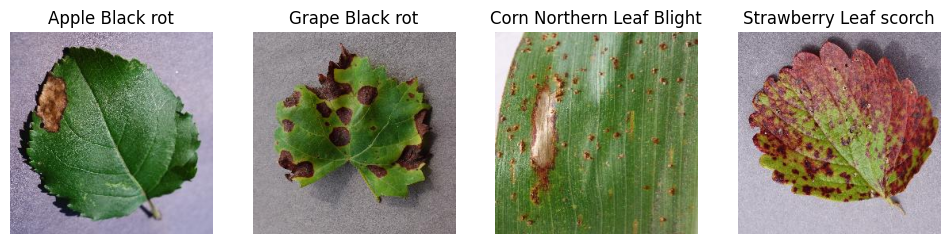
\includegraphics[width=15cm]{../../images/example_images_of_plantvillage.png}
    \caption{Example images of the \gls{pvd}}\label{fig:example_images_of_plantvillage}
    \end{center}
\end{figure}
With 54'303 images it is one of the larger plant disease data sets available. Accordingly, it is often used in other work \autocite{hughes2016}, but there is no official test split provided to compare the results of already existing models. Some achieved an accuracy around 90\% with the ResNet50 architecture \autocite{gole2023}.
The data set includes different plants such as apple and tomatoes, but also different plant diseases. Some diseases like ``tomato early blight'' and ``potato early blight'' have the same root cause, but the symptoms look a bit different. 
The splitting was carried out by myself using 80\% of the data for the training set and 10\% each for the validation and test set. The stratifying ensures, that the distribution of the 38 classes is the same over all sets, which can be seen in Figure~\ref{fig:class_distribution_of_plantvillage}.
\begin{figure}[H]
    \begin{center}
    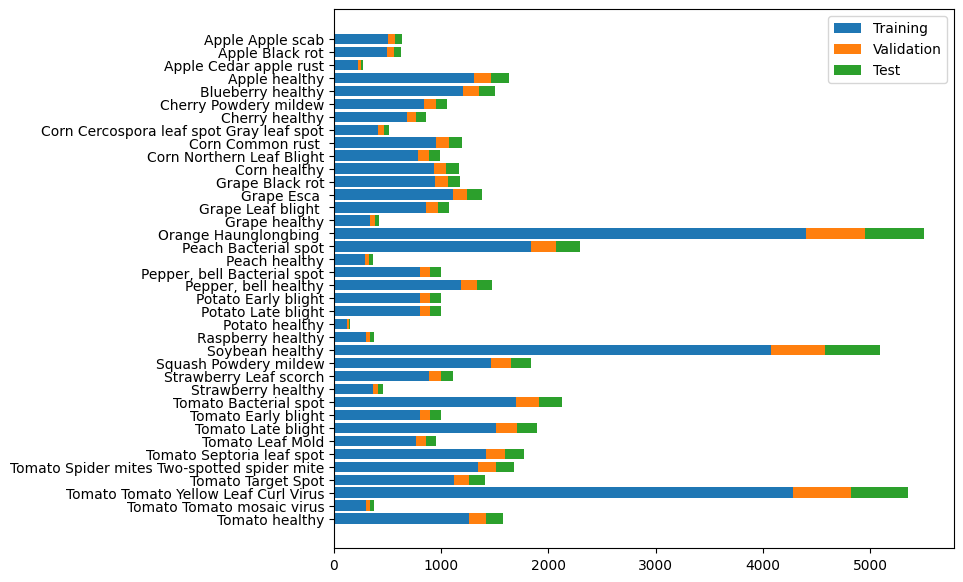
\includegraphics[width=15cm]{../../images/class_distribution_of_plantvillage.png}
    \caption{Class distribution of PlantVillage}\label{fig:class_distribution_of_plantvillage}
    \end{center}
\end{figure}

\subsection{Cassava Leaf Disease Classification}
The data set contains 21'398 of cassava leaves with a natural background as visible in Figure~\ref{fig:example_images_of_cassava}.
\begin{figure}[H]
    \begin{center}
    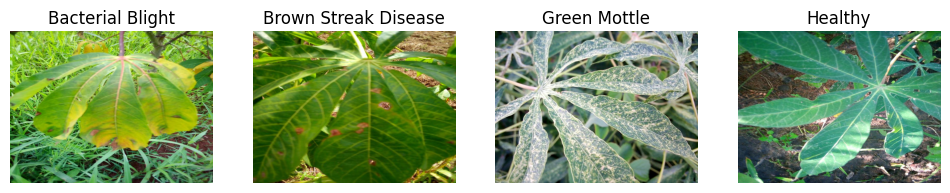
\includegraphics[width=15cm]{../../images/example_images_of_cassava.png}
    \caption{Example images of the cassava dataset}\label{fig:example_images_of_cassava}
    \end{center}
\end{figure}
Kaggle possesses a non-public test set with which submitted notebooks get tested \autocite{mwebaze2020}. Currently, the best result has an accuracy of roughly 91\% and is achieved with an ensemble model containing a Resnet50, \gls{vit} and further models.  
The split for this work was also done by myself, resulting in the distribution shown in Figure~\ref{fig:class_distribution_of_cassava}.
\begin{figure}[H]
    \begin{center}
    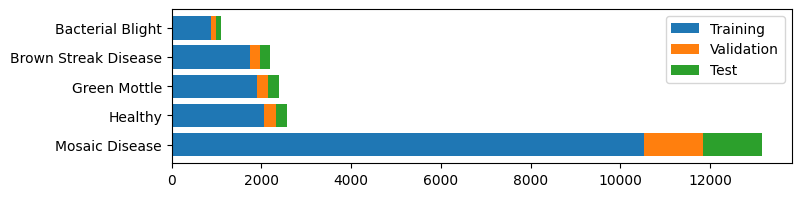
\includegraphics[width=15cm]{../../images/class_distribution_of_cassava.png}
    \caption{Class distribution of Cassava}\label{fig:class_distribution_of_cassava}
    \end{center}
\end{figure}
It is noticeable that the ``Mosaic Disease'' dominates over the other classes. A baseline score was calculated for all downstream tasks. This score corresponds to the result when the model is only assigning the most common as prediction for all data points. The complete list of these baseline values is listed in the Appendix~\ref{appendix:baseline_scores}

\subsection{PlantDataset}
The origin of the PlantDataset is not exactly known. The data is available on the kaggle platform, but it is unclear what it is intended for exactly. As far as is known, it is not used in any paper either.
The images do not only contain leaves, but also the bark or fruits for some classes as depicted in Figure~\ref{fig:example_images_of_plantdataset}.
\begin{figure}[H]
    \begin{center}
    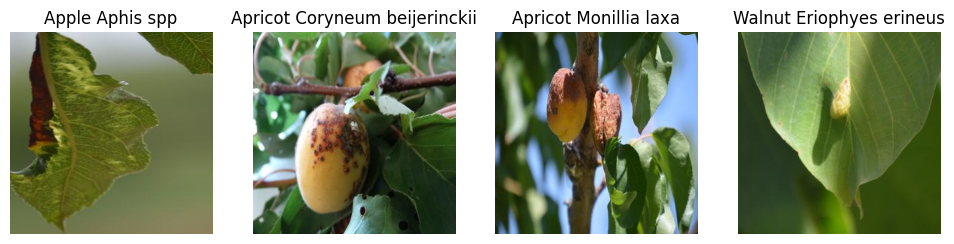
\includegraphics[width=15cm]{../../images/example_images_of_plantdataset.png}
    \caption{Example images of PlantDataset}\label{fig:example_images_of_plantdataset}
    \end{center}
\end{figure}
A small disadvantage of this data set is the presence of near duplicates in some classes. This should not be a problem, as most classes are safe.

Figure~\ref{fig:class_distribution_of_plantdataset}
\begin{figure}[H]
    \begin{center}
    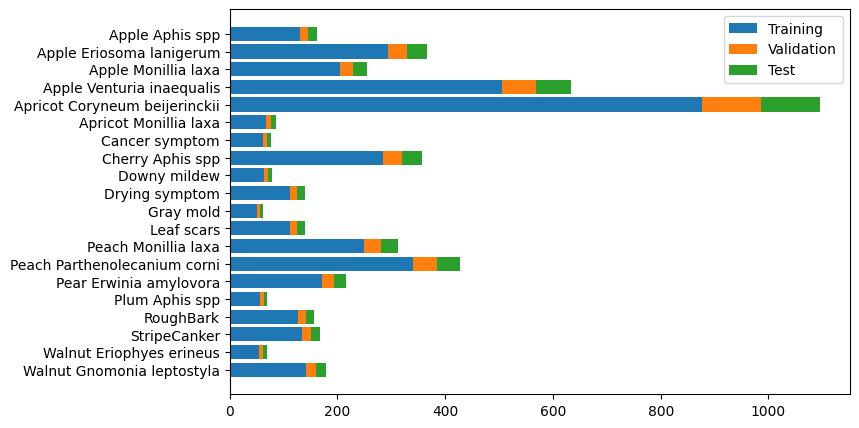
\includegraphics[width=15cm]{../../images/class_distribution_of_plantdataset.png}
    \caption{Class distribution of PlantDataset}\label{fig:class_distribution_of_plantdataset}
    \end{center}
\end{figure}

\subsection{PlantDoc}
This data set was chosen, because it contains a wild mix of images scrapped from the internet. Figure~\ref{fig:example_images_of_plantdoc} shows, that some pictures even have a watermark on them or some.
\begin{figure}[H]
    \begin{center}
    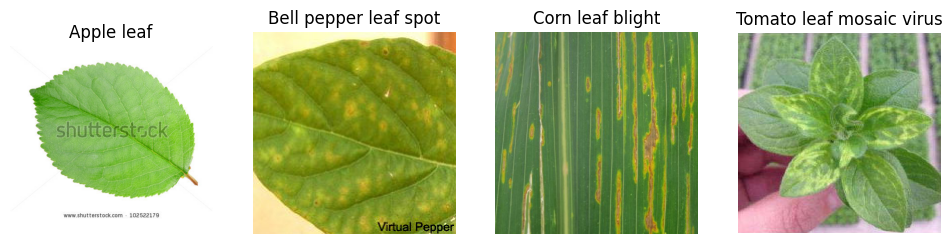
\includegraphics[width=15cm]{../../images/example_images_of_plantdoc.png}
    \caption{Example images of PlantDoc}\label{fig:example_images_of_plantdoc}
    \end{center}
\end{figure}
The corresponding paper lists the achieved scores. The best accuracy and f1-score are roughly 70\% \autocite{singh2020}. The data set contains some falsely classified images, which was also confirmed by the creators. For this work these few errors should not be a problem, because the classification of the plants is not as important as detecting the stains.
The 2'598 images are distributed as shown in Figure~\ref{fig:class_distribution_of_plantdoc}.

\begin{figure}[H]
    \begin{center}
    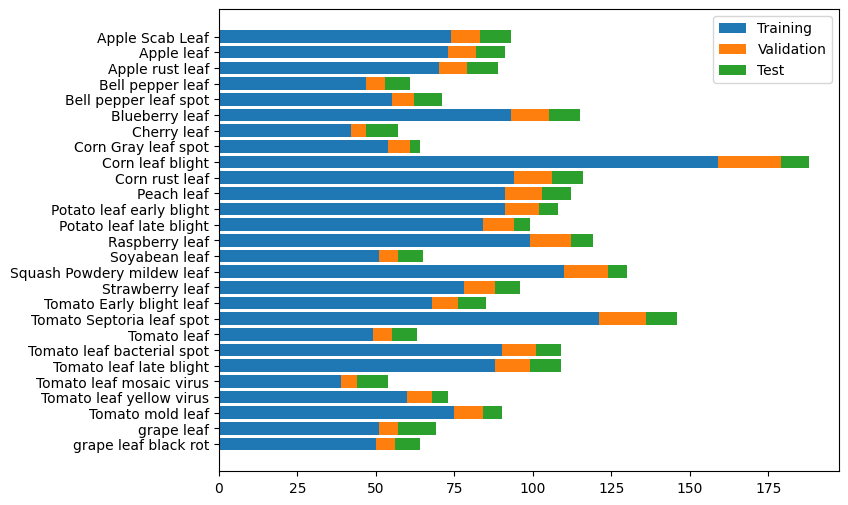
\includegraphics[width=15cm]{../../images/class_distribution_of_plantdoc.png}
    \caption{Class distribution of PlantDoc}\label{fig:class_distribution_of_plantdoc}
    \end{center}
\end{figure}

\section{SSL plant datasets}

Due to their size, the following data sets were not used as downstream tasks, but only to create a plant based \gls{ssl} model. 
\subsection{DARMA}
The \gls{darma} has a total of 231'414 and 1000 different plant classes rather than diseases. It also includes images of other plant parts than leaves like bark or blossoms. Figure~\ref{fig:example_images_of_darma} shows some of such examples.

\begin{figure}[H]
    \begin{center}
    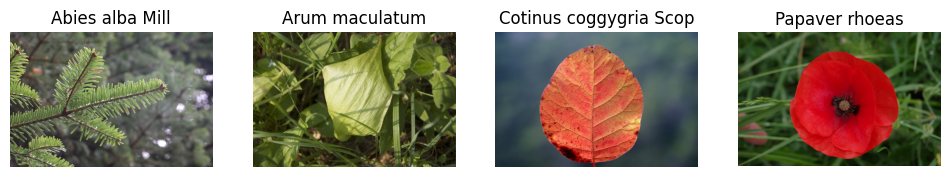
\includegraphics[width=15cm]{../../images/example_images_of_darma.png}
    \caption{Example images of \gls{darma}}\label{fig:example_images_of_darma}
    \end{center}
\end{figure}

\subsection{Plant Disease Diagnosis Dataset (PDDD)}
The \gls{pddd} contains 421'133 pictures of diseased plants, which is an ideal addition to the more generic images of \gls{darma}.
A few example images are shown in Figure~\ref{fig:example_images_of_pddd}. Some of its classes are also present in the downstream tasks making it a promising basis.
\begin{figure}[H]
    \begin{center}
    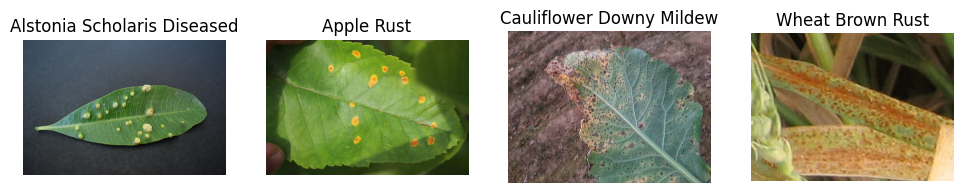
\includegraphics[width=15cm]{../../images/example_images_of_pddd.png}
    \caption{Example images of \gls{pddd}}\label{fig:example_images_of_pddd}
    \end{center}
\end{figure}

This large-scale plant disease dataset is explicitly meant to be used to pre-train models that then can be fine-tuned on specific downstream tasks \autocite{dong2023}. They also provide a brad selection of \gls{sl} trained models to be used for fine-tuning. This work uses the provided weights of the Resnet50 model to compare its performance on plant and dermatology tasks.

Although weights for the Resnet50 architecture are provided, there are no 

\section{Dermatology datasets}\label{section:derma_datasets}
%TODO
% The following data sets are selected by F.~Gröger due to his former experience.

\begin{table}[H]
    \centering
    \caption{Dermatology datasets\label{tab:suitable_derma_datasets}}
    \begin{tabularx}{\textwidth}{|
        >{\hsize=.72\hsize}X |
        >{\hsize=.14\hsize\raggedleft}X |
        >{\hsize=.14\hsize\raggedleft}X |
}
\hline
\textbf{Name} & \textbf{\#Images} & \textbf{\#Classes} \tabularnewline \hline
\gls{ddi} \autocite{daneshjou2022} & 656 & 2, 78 \tabularnewline \hline
PAD-UFES-20 \autocite{pacheco2020} & 2'298 & 6 \tabularnewline \hline
HAM10000 \autocite{codella2019,tschandl2018} & 10'015 & 7 \tabularnewline \hline
Fitzpatrick17k \autocite{groh2021} & 16'536 & 9,3 \tabularnewline \hline
\end{tabularx}
\end{table}

\subsection{Diverse Dermatology Images (DDI)}
\gls{ddi} is the smallest dataset with only 656 images. Instead of using the detailed classes the main classification into malignant and non-malignant is made.
Figure~\ref{fig:example_images_of_ddi} shows, that the classification of many cases is not obvious.
\begin{figure}[H]
    \begin{center}
    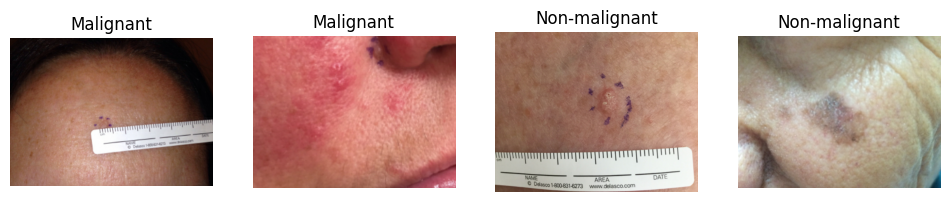
\includegraphics[width=15cm]{../../images/example_images_of_ddi.png}
    \caption{Example images of \gls{ddi}}\label{fig:example_images_of_ddi}
    \end{center}
\end{figure}

The binary classes, visible in Figure~\ref{fig:class_distribution_of_ddi}, are skewed. This leads to a high baseline values for this data set, listed in the Appendix~\ref{appendix:baseline_scores}.

\begin{figure}[H]
    \begin{center}
    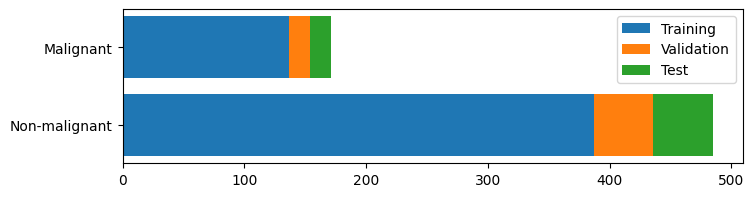
\includegraphics[width=15cm]{../../images/class_distribution_of_ddi.png}
    \caption{Class distribution of \gls{ddi}}\label{fig:class_distribution_of_ddi}
    \end{center}
\end{figure}


\subsection{PAD-UFES-20}
The PAD-UFES-20 data set provide 2'298 images of skin lesions belonging to six different classes. 
Figure~\ref{fig:example_images_of_pad-ufes-20} lists some example images.

\begin{figure}[H]
    \begin{center}
    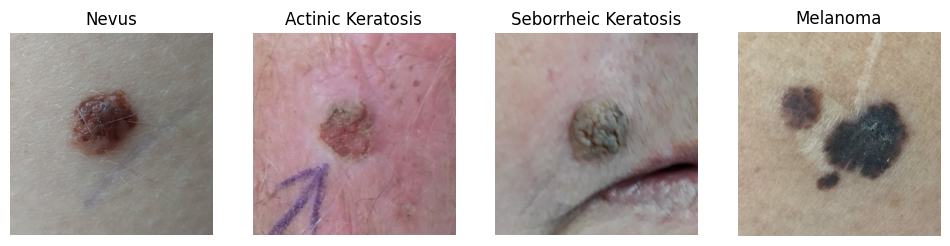
\includegraphics[width=15cm]{../../images/example_images_of_pad-ufes-20.png}
    \caption{Example images of PAD-UFES-20}\label{fig:example_images_of_pad-ufes-20}
    \end{center}
\end{figure}

Every image also has a patient id. This patient id was considered while dividing the data into subsets. As visible in Figure~\ref{fig:class_distribution_of_pad-ufes-20} the distribution is still similar in the subsets. 

\begin{figure}[H]
    \begin{center}
    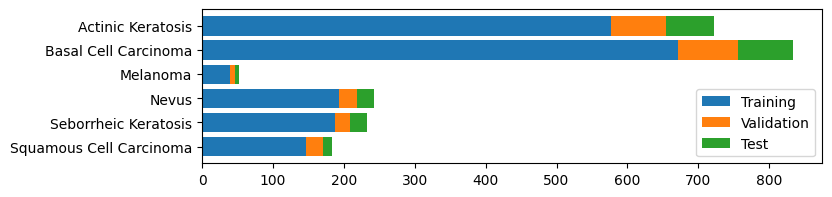
\includegraphics[width=15cm]{../../images/class_distribution_of_pad-ufes-20.png}
    \caption{Class distribution of PAD-UFES-20}\label{fig:class_distribution_of_pad-ufes-20}
    \end{center}
\end{figure}


\subsection{HAM10000}
The HAM10000 dataset is based on the \gls{isic} 2018 challenge \autocite{codella2019}. The \gls{ssl} pre-training of the dermatology model also used images from \gls{isic}. The effects caused by similar data should in that case be the most clearly.
Figure~\ref{fig:example_images_of_ham10000} shows the uniformity of the picture. The affected area is always centered and clearly visible.
\begin{figure}[H]
    \begin{center}
    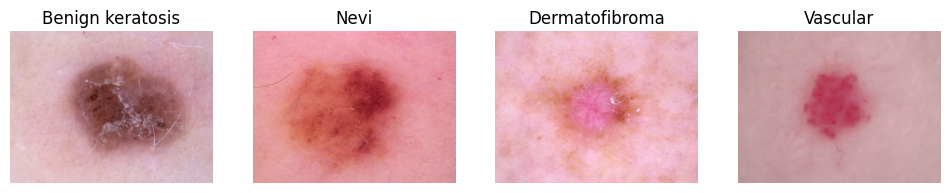
\includegraphics[width=15cm]{../../images/example_images_of_ham10000.png}
    \caption{Example images of HAM10000}\label{fig:example_images_of_ham10000}
    \end{center}
\end{figure}
HAM10000 comes with a predefined test split. This does only influence the split as visible in Figure~\ref{fig:class_distribution_of_ham10000}.
Additionally, the class ``Nevi'' dominates the other classes. Lastly the two classes ``Dermatofibroma'' and ``Vascular'' do not have enough samples for subsampling 30 data points per class.
\begin{figure}[H]
    \begin{center}
    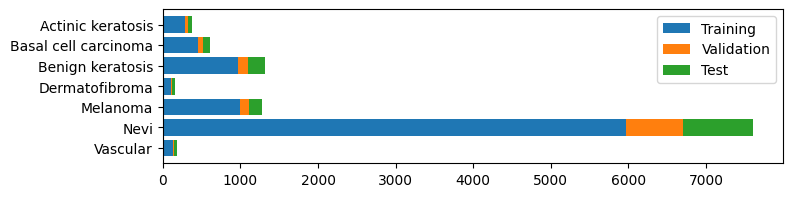
\includegraphics[width=15cm]{../../images/class_distribution_of_ham10000.png}
    \caption{Class distribution of HAM10000}\label{fig:class_distribution_of_ham10000}
    \end{center}
\end{figure}


\subsection{Fitzpatrick17k}
With 16'536 images is Fitzpatrick17k the largest dermatology data set in this work. The Different areas of skin can be affected as seen in Figure~\ref{fig:example_images_of_fitzpatrick17k}.

\begin{figure}[H]
    \begin{center}
    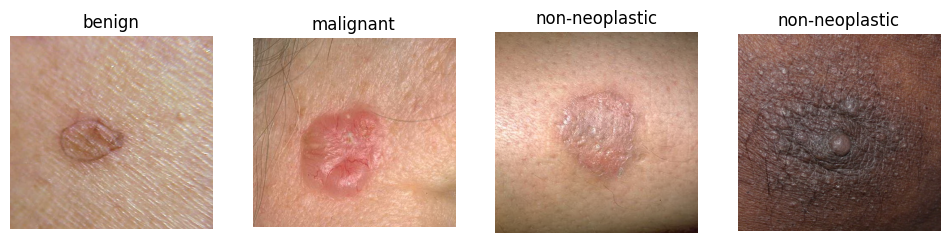
\includegraphics[width=15cm]{../../images/example_images_of_fitzpatrick17k.png}
    \caption{Example images of Fitzpatrick17k}\label{fig:example_images_of_fitzpatrick17k}
    \end{center}
\end{figure}

Beside \gls{ddi} this data set also provides more than one possible target class. In this work the following three classes were used. This can also be seen on Figure~\ref{fig:class_distribution_of_fitzpatrick17k}.

\begin{figure}[H]
    \begin{center}
    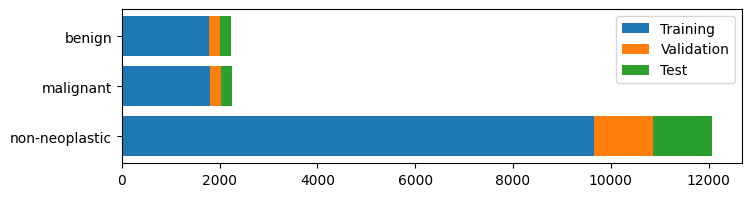
\includegraphics[width=15cm]{../../images/class_distribution_of_fitzpatrick17k.png}
    \caption{Class distribution of Fitzpatrick17k}\label{fig:class_distribution_of_fitzpatrick17k}
    \end{center}
\end{figure}

\subsection{SSL dermatology datasets}
The pre-trained dermatology models were provided by Fabian Gröger from a previous work \autocite{groeger2023}. Images from following data sets were used for training.


\begin{itemize}
    \item MED-NODE: 170'462 clinical images \autocite{giotis2015}
    \item PH2 Database: 200 dermoscopy images \autocite{mendonca2013}
    \item Derm7pt: 2'022 images \autocite{kawahara2019}
    \item SD-260: 12'583 clinical images \autocite{sun2016}
    \item ISIC: 107'208 images \autocite{giotis2015}
    \item A private collection of roughly 120'000 clinical images 
\end{itemize}
